\section{Аналитическая часть}

В данной части проводится анализ объектов сцены и существующих алгоритмов построения изображений и выбор более подходящих алгоритмов для дальнейшего использования.

\subsection{Формализация объектов синтезируемой сцены}

Сцена состоит из определенного набора объектов.
\begin{enumerate}
	\item Направленный источник света представляет собой вектор направления света и принимает ортогональную проекцию визуализируемой сцены из своего положения с некоторым ограниченным положением. В зависимости от расположения источника и направления распространения лучей света, определяется тень от объекта, расположенных на сцене. Цвет свечения описывается через RGB параметры.
	\item Объекты сцены -- примитивные многогранники, расположенные в пространстве сцены. Каждая модель многогранника представляет собой набор граней, описываемых точками в пространстве, которые соединены ребрами и задается параметрическими (радиус нижнего и верхнего основания, количество боковых граней и высота) и спектральными характеристиками (зеркальный коэффициент, коэффициент блеска и цвет) для построения. 
	\item Камера характеризуется своим пространственным положением и направлением просмотра.
\end{enumerate}

\subsection{Способы описания трехмерных геометрических моделей на сцене}

В компьютерной графики для описание трехмерных геометрических объектов существует три типа моделей: каркасная, поверхностная и твердотельная~\cite{aaymodelmethod}. Использование моделей позволяет правильно отображать форму и размеры объектов сцены.

\begin{itemize}
	\item \textit{Каркасная модель} --- простейший вид моделей, который содержит минимум информации только о вершинах и ребрах объектов. Это моделирование самого низкого уровня, которое имеет ряд серьезных ограничений, большинство из которых возникает из-за недостатка информации о гранях, которые заключены между ребрами. Невозможно выделить внутреннюю и внешнюю область изображения твердого объемного тела. Однако каркасная модель требует меньше памяти и затрат времени на построение, что достаточно пригодна для решения задач, не требующие информации о поверхности объекта (например, если в объекте есть отверстия). Проблемой этой модели заключается в том, что она не позволяет отличить видимые грани от невидимых. Операции по удалению невидимых линий можно выполнить только вручную с применением команд редактирования каждой отдельной линии, но результат работы нарушает каркасную конструкцию, по причине того что линии невидимы в одном случае и видимы в другом.
	Кроме того, каркасная модель не несет информации о поверхностях, ограничивающих форму, что обуславливает невозможность обнаружения нежелательных взаимодействий между гранями объекта~\cite{roders}.
	\item \textit{Поверхностная модель} часто используется в компьютерной графике, кроме содержание информации о вершинах и ребрах, содержит еще информацию о поверхности. При построении поверхностной модели предполагается, что технические объекты ограничены поверхностями, которые отделяют их от окружающей среды. 
	Недостатком поверхностной модели является отсутствие информации о том, с какой стороны поверхности находится материал.
	\item \textit{Твердотельная модель} отличается от поверхностной тем, что в данной модели к информации о поверхностях добавляется информация о том, с какой стороны расположен материал. Это достигается путем указания направления внутренней нормали.
\end{itemize}

Для решения поставленной задачи не подойдет каркасная модель, так как такое представление будет приводить к неправильному восприятию форм объекта. Твердотельная модель также не подойдет, так как по поставленной задачи нет необходимости знать из какого материала будет выполнен тот или иной объект и с какой стороны расположен материал. Поэтому выбор остается лишь поверхностной модели.

\subsection{Способы задания поверхностных моделей}

Поверхностная модель задается следующими способами~\cite{roders, porev}.
\begin{itemize}
	\item \textit{Аналитический (параметрический) способ} характеризуется описанием модели объекта, которое доступно в неявной форме,то есть для получения визуальных характеристик необходимо дополнительно вычислять некоторую функцию, которая зависит от параметра, что в свою очередь довольно удобно при просчете поверхностей вращения. 
	\item \textit{Полигональная сетка} характеризуется совокупностью вершин, ребер и граней, определяющих форму объекта в трехмерном пространстве.
\end{itemize}

\begin{figure}[h]
	\centering
	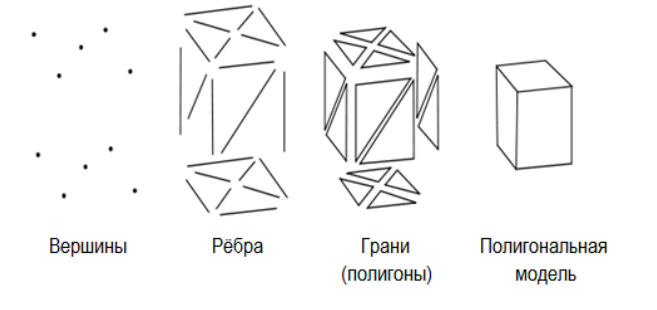
\includegraphics[height=0.3\textheight]{img/polygonal-grid.png}
	\caption{Полигональная сетка}
	\label{img:polygonal-grid}
\end{figure}

Рассмотрим существующие способы хранения информации о полигональной сетке.

Вершинное представление описывает объект множество вершин, соединенных с другими вершинами (вершины, которые указывают на другие вершины). 
Информация о ребрах и гранях неявно присутствует в представлении из-за чего для восстановления исходного тела необходимо обойти все вершины и составить списки граней. 
Кроме того, операции с ребрами и гранями выполнить нелегко~\cite{aaymodelmethod}.
Тем не менее из-за простоты представления дает возможность множество операций над сеткой. 
Хранение информации о сетке требует не так много памяти по сравнению с другими способами.
На рисунке~\ref{img:vertex-method} представлен пример вершинного представления, рассмотренный на кубе.

\begin{figure}[h]
	\centering
	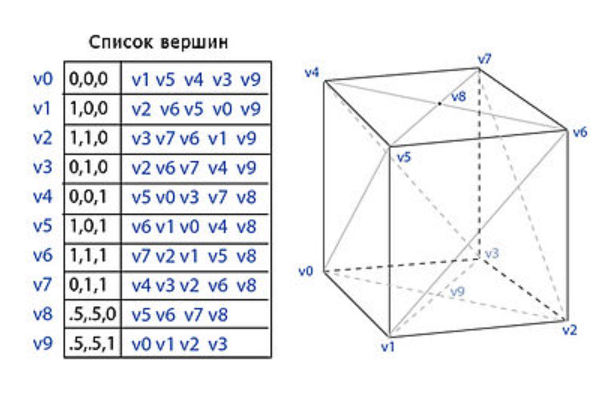
\includegraphics[height=0.3\textheight]{img/vertex-method.png}
	\caption{Вершинное представление}
	\label{img:vertex-method}
\end{figure}

Представление называемый списком граней представляет объект не только множеством вершин, но граней. 
В отличие от предыдущего способа, вершины и граны определены явно, благодаря чему нахождение соседних вершин и граней довольно проста и поиск соседних граней и вершин занимает постоянное время~\cite{aaymodelmethod}. 
Также список вершин содержит список граней, связанных с каждой вершиной. 
Однако ребра неявны, поэтому поиск все равно необходим, чтобы найти все грани, окружающие данную грань. 
Другие динамические операции, такие как разделение или слияние граней, также сложны с сетками граней и вершин. 
Пример представления список граней представлен на рисунке~\ref{img:list-faces}.

\begin{figure}[h]
	\centering
	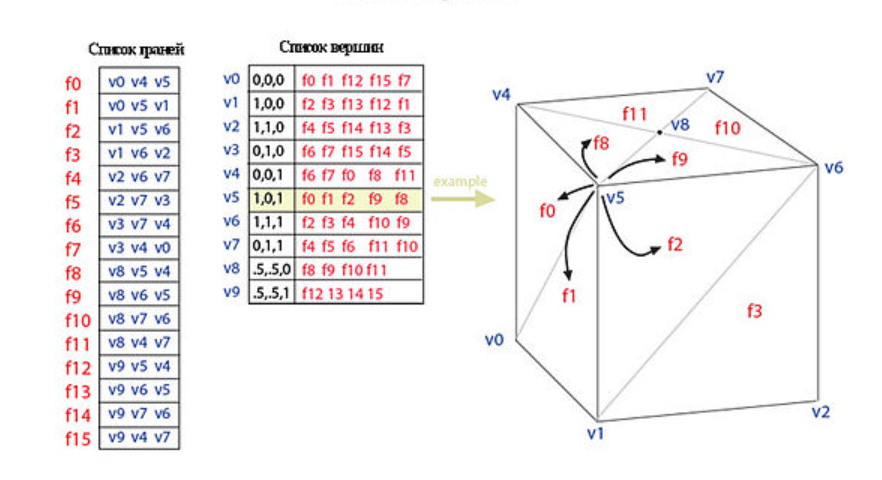
\includegraphics[height=0.3\textheight]{img/list-faces.png}
	\caption{Список граней}
	\label{img:list-faces}
\end{figure}

Представление называемый таблицей углов представляет специальной таблицей, хранящей вершины, обход которых неявно задает полигоны. 
Такое представление более компактно и более производительно для нахождение полигонов, но в связи с тем, что вершины присутствуют в описании нескольких углов, операции по их изменению медленны. 
Также угловые таблицы представляют сетки не полностью, из-за чего их требуется несколько.

<<Крылатое>> представление задает точки, каждая из которых указывает на две вершины, две грани и четыре ребра, которые ее касаются, благодаря чему обход поверхностей выполняется за постоянное время. 
Однако метод очень требует памяти и изменения геометрических характеристик приводит к формированию списка индексов граней.
Данный способ полезен для определения столкновений объектов. 
Пример представлен на рисунке~\ref{img:winged-method}.

\begin{figure}[h]
	\centering
	\includegraphics[height=0.5\textheight]{img/winged-method.png}
	\caption{<<Крылатое>> представление}
	\label{img:winged-method}
\end{figure}

Оптимальное для реализации представление многогранника --- модель, заданная полигональной сеткой. 
Такая модель позволит избежать проблем при описании сложных объектов сцены. 
Способом хранения полигональной сетки был выбран список граней, так как это даст явное описание граней. 
Этот способ позволит эффективно преобразовывать модели, так как структура будет включать в себя список вершин.

\subsection{Анализ алгоритмов удаления невидимых линий и поверхностей}

Основной задачей при построении реалистичного изображения является задача удаления объектов или их частей, которые перекрываются другими объектами, то есть являются невидимыми с точки зрения наблюдателя. Выделяют две группы алгоритмов для ее решения:
\begin{itemize}
	\item Алгоритмы, работающие в объектном пространстве. Данные алгоритмы имеют привязку к мировой или физической системе координат. Получаемые результаты ограничиваются только точностью вычислений, однако требуют большого объема вычислений, зависящего от требуемой точности и сложности поступающей на вход сцены. В эту группу входят алгоритм Робертса, алгоритм со списком приоритетов и т.д.~\cite{roders} 
	\item Алгоритмы, работающие в пространстве изображения. Данные алгоритмы предполагают привязку к системе координат экрана или картинной плоскости, на которую производится проецирование изображаемых объектов. Объем требуемых вычислений значительно меньше, чем у алгоритмов первой группы, и зависит от разрешающей способности экрана и количества объектов на сцене. Основными представителями данной группы являются алгоритм Варнака, алгоритм Z-буфера и алгоритм трассировки лучей~\cite{roders}. 
\end{itemize}


\subsubsection{Алгоритм Робертса}

Данный алгоритм работает в объектном пространстве, решая задачу только с выпуклыми телами, и выполняется в 3 этапа~\cite{roders}. 

Первый этап --- подготовка исходной матрицы $V$, которая задает информацию о каждой фигуре. 
Размерность матрицы -- $4 * n$, где $n$ -- количество граней тела.
Каждый столбец матрицы представляет собой четыре коэффициента уравнения плоскости $ax + by + cz + d = 0$, проходящей через очередную грань.
Таким образом, матрица тела будет представлена в следующем виде:
\begin{equation}
	V = \begin{pmatrix}
		a_{1} & a_{2} & \ldots & a_{n}\\
		b_{1} & b_{2} & \ldots & b_{n}\\
		c_{1} & c_{2} & \ldots & c_{n}\\
		d_{1} & d_{2} & \ldots & d_{n}
	\end{pmatrix}
\end{equation}
Матрица тела должна быть сформирована корректно, то есть любая точка, расположенная внутри тела, должна располагаться по положительную сторону от каждой грани тела. 
В случае, если для очередной грани условие не выполняется, соответствующий столбец матрицы надо умножить на $-1$. 
Для проведения проверки следует взять точку, расположенную внутри тела. 
Координаты такой точки можно получить путем усреднения координат всех вершин тела.

Второй этап --- удаления ребер, экранируемых самим телом, где рассматривается вектор взгляда $E = \{0, 0, -1, 0\}$.
Для определения невидимых граней достаточно умножить вектор $E$ на матрицу тела $V$. 
Отрицательные компоненты полученного вектора будут соответствовать невидимым граням.

Третий этап --- удаление невидимых ребер, экранируемых другими телами сцены. 
Для определения невидимых точек ребра требуется построить луч, соединяющий точку наблюдения с точкой на ребре. 
Точка будет невидимой, если луч на своем пути встречает в качестве преграды рассматриваемое тело. 
Если тело является преградой, то луч должен пройти через тело. 
Если луч проходит через тело, то он находится по положительную сторону от каждой грани тела.

В данном алгоритме главным недостатком является его вычислительная трудоемкость равная $O(n^2)$, где $n$ --- количество объектов на сцене. Также все тела на сцене должны быть выпуклыми, что приводит к дополнительным проверкам.
Однако, работа в объектном пространстве и высокая сложность вычислений обеспечивает высокую точность результата.

\subsubsection{Алгоритм Варнока}

Алгоритм Варнока работает в пространстве изображения и позволяет определить, какие грани или части граней объектов сцены видимы, а какие заслонены другими объектами~\cite{roders, shikin}. 
Алгоритм прелагает разбиение области изображения на более мелки окна, и для каждого такого окна определяются связанные с ней многоугольники и те, видимость которых можно определить, изображаются на сцене.
На рисунке~\ref{img:varnok} представлен пример разбиние с помощью алгоритма Варнака.

\begin{figure}[h]
	\centering
	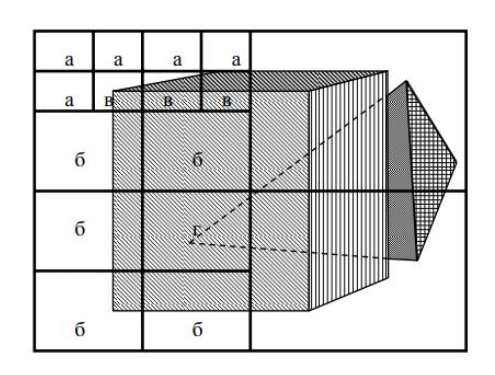
\includegraphics[height=0.25\textheight]{img/varnok.png}
	\caption{Пример разбиения алгоритмом Варнака}
	\label{img:varnok}
\end{figure}

В качестве граней обычно выступают выпуклые многоугольники, алгоритмы работы с ними эффективнее, чем с произвольными многоугольниками.
Окно, в котором необходимо отобразить сцену, должно быть прямоугольным. 
Алгоритм работает рекурсивно, что является его главным недостатком, на каждом шаге анализируется видимость граней и, если нельзя <<легко>> определить видимость, окно делится на 4 части и анализ повторяется отдельно для каждой из частей. 

\subsubsection{Алгоритм, использующий Z-буфер}

Алгоритм, использующий z-буфер, является одним из самых простых и широко используемых и работает в пространстве изображения.
Идея z-буфер является простым обобщением идеи о буфере кадра~\cite{roders}.
Используется два буфера:
\begin{itemize}
	\item буфер кадра, который используется для запоминания атрибутов (интенсивности) каждого пиксела;
	\item z-буфер --- отдельный буфер глубины, используемый для запоминания координаты z каждого пиксела.
\end{itemize}

Первоначально в z-буфере находятся минимально возможные значения z, а в буфере кадра располагаются пиксели, описывающие фон.
В процессе работы глубина z каждого нового пиксела, который нужно занести в буфер кадра, сравнивается с глубиной того пиксела, который уже занесен в z-буфер.
Если новый пиксель расположен ближе к наблюдателю, чем предыдущий, то он заносится в буфер кадра и происходит корректировка z-буфера. Затем каждый многоугольник преобразуется в растровую форму и записывается в буфер кадра, при этом не производится начального упорядочения
В противном случае никаких действий не производится~\cite{roders}.
На рисунке~\ref{img:z-buffer} представлена пример работы алгоритма Z-буфера.
\begin{figure}[h]
	\centering
	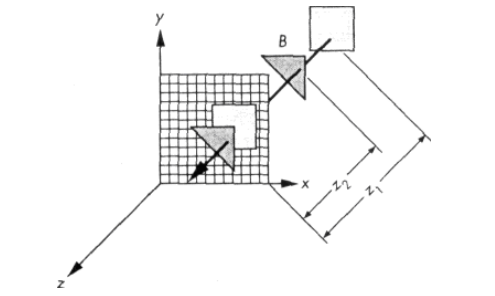
\includegraphics[height=0.3\textheight]{img/z-buffer.png}
	\caption{Алгоритм с Z-буфером}
	\label{img:z-buffer}
\end{figure}

Основным преимущество алгоритма является простота реализации.
Трудоемкость алгоритма увеличивается линейно в зависимости от количества объектов на сцене.
Особая эффективность по времени достигается за счет того, что нет необходимости в сортировки объектов. 
Это является большим плюсом, так как на сцене может быть большое количество объектов.
Однако алгоритм очень требователен к памяти из-за необходимости хранить информацию о каждом пикселе и выделение памяти под два буфера.
Реализация эффектов прозрачности и устранения лестничного эффекта осложнена.

\subsubsection{Алгоритм прямой трассировки лучей}

Главная идея, лежащая в основе алгоритма трассировки лучей, заключается в том, что наблюдатель видит любой объект посредством испускаемого неким источником света, который падает на этот объект и затем согласно законам оптики некоторым путем доходит до глаза наблюдателя. 
В методе прямой трассировки предполагает построения траекторий лучей от всех источников света ко всем точкам всех объектов сцены, отражаются и преломляются или проходят сквозь него и в результате достигает наблюдателя.
Данные лучи называются первичными.
Если объект не является отражающим или прозрачным, то траектория луча на этой точке обрывается~\cite{roders, ray-tracing}.

\begin{figure}[h]
	\centering
	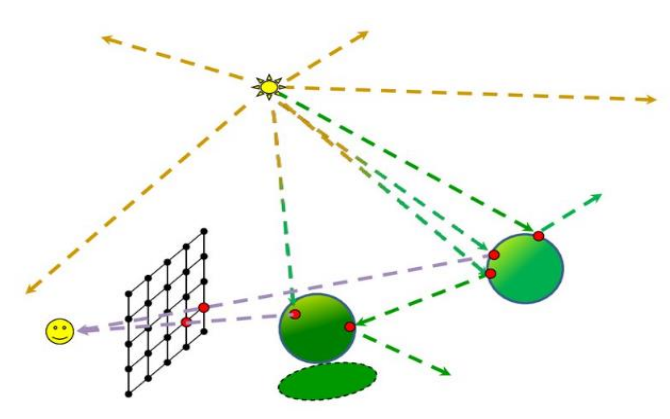
\includegraphics[height=0.25\textheight]{img/direct-ray-tracing.png}
	\caption{Алгоритм прямой трассировки лучей}
	\label{img:ray-tracing}
\end{figure}

Основным недостатком алгоритма является излишне большое число рассматриваемых лучей, приводящее к существенным затратам вычислительных мощностей, так как лишь малая часть лучей достигает точки наблюдения.
Данный алгоритм подходит для генерации статических сцен и моделирования зеркального отражения, а так же других оптических эффектов как отражение, преломление и т.д.

\subsubsection{Алгоритм обратной трассировки лучей}

Наблюдатель видит объект посредством испускаемого источником света,
который падает на этот объект и согласно законам оптики некоторым путем доходит до глаза наблюдателя. Отслеживать пути лучей от источника к наблюдателю неэффективно с точки зрения вычислений, поэтому наилучшим способом будет отслеживание путей в обратном направлении, то есть от наблюдателя к объекту. 
Лучи испускаются из камеры, пронизывая каждый пиксель сцены. 
После этого определяют пересечение первичного луча с объектами сцены. 
Первичный луч – луч, выпущенный из камеры. 
Если оно было установлено, вычисляют интенсивность пиксела, учитывая положения источников света~\cite{roders, ray-tracing}.

\begin{figure}[h]
	\centering
	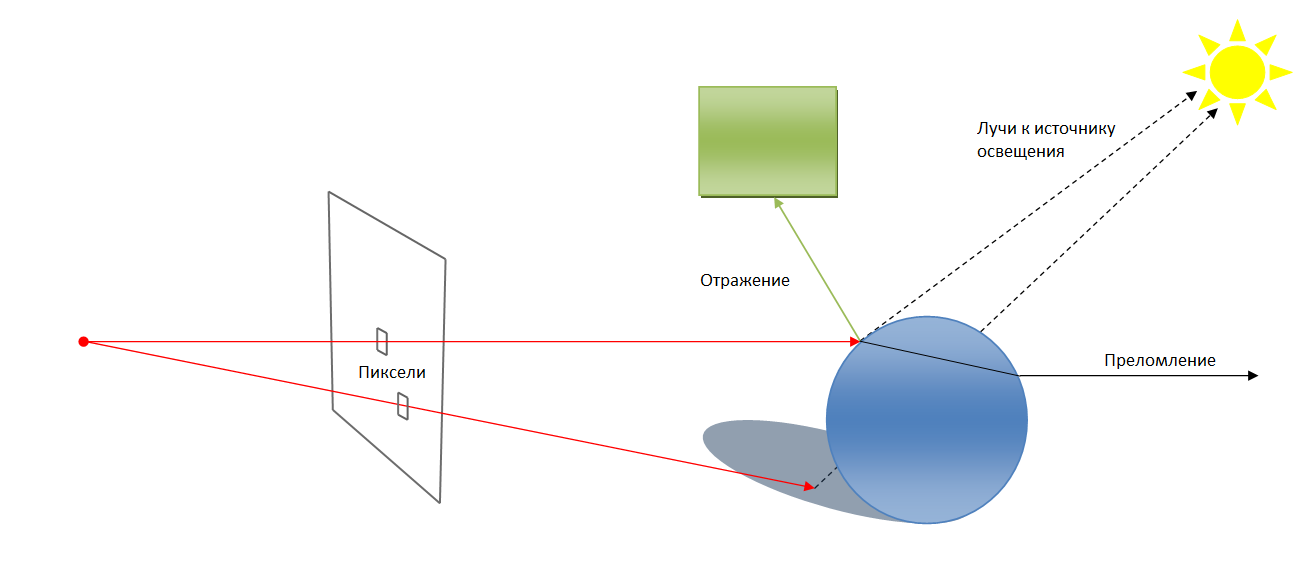
\includegraphics[height=0.25\textheight]{img/reverse-ray-tracing.png}
	\caption{Алгоритм обратной трассировки лучей}
	\label{img:rray-tracing}
\end{figure}

Считается, что наблюдатель расположен на положительной полуоси $z$ в бесконечности, поэтому все световые лучи параллельны оси $z$. 
В ходе работы испускаются лучи от наблюдателя и ищутся пересечения луча и всех объектов сцены. 
В результате пересечение с максимальным значением $z$ является видимой частью поверхности и атрибуты данного объекта используются для определения характеристик пиксела, через центр которого проходит данный
световой луч.
Для расчета эффектов освещения сцены проводятся вторичные лучи от точек пересечения ко всем источникам света. Если на пути этих лучей встречается непрозрачное тело, значит, данная точка находится в тени.

Несмотря на более высокую эффективность алгоритма в сравнении с прямой трассировкой лучей, данный алгоритм считается достаточно медленным, так как в нем происходит точный расчет сложных аналитических выражений для нахождения пересечения с рассматриваемыми объектами~\cite{shikin}.

\subsubsection{Выбор оптимального алгоритма}

При реализации редактора композиций из графических примитивов многогранников необходимо обеспечить плавную смену кадров при перемещении камеры и изменении объектов, поэтому алгоритм должен иметь минимальную зависимость трудоемкости алгоритма от числа объектов на сцене и использование рекурсивных вызовов. Также требуется учесть ограничение разработки  курсового проекта, поэтому требуется простота реализации алгоритма. Задействования дополнительной памяти под буферы не является весомым критерием и может быть опущен.

Таким образом, подходящий алгоритм является алгоритм с Z-буфером, который подходит для решения создания сцены с различным количеством объектов, что позволит иметь динамическую сцену.
Данный алгоритм имеет линейную зависимость от числа объектом, что приведет к оптимальной работе программы.
Также он простой в реализации и используется в большинстве графических движков, что приведет к быстрой скорости реализации алгоритма.

\subsection{Анализ алгоритмов закраски}

Методы закраски используются для затенения полигонов модели в условиях некоторой сцены, имеющей источники освещения.
Учитывая взаимное положение рассматриваемого полигона и источника света, можно найти уровень освещенности по закону Ламберта~\cite{roders}:
\begin{equation}
	\label{for:lambert}
	I_{\alpha} = I_0 \cdot \cos{(\alpha)},
\end{equation}
где $I_{\alpha}$ - уровень освещенности в рассматриваемой точке, $I_0$ - максимальный уровень освещенности, а $\alpha$ - угол между вектором нормали к плоскости и вектором, направленным от рассматриваемой точки к источнику освещения.

Существует три основных алгоритма, позволяющих закрасить полигональную модель.

\subsubsection{Простая закраска}

Вся грань закрашивается одним уровнем интенсивности, который высчитывается по закону Ламберта. При данной закраске все плоскости (в том числе и те, что аппроксимируют фигуры вращения), будут закрашены однотонно, что в случае с фигурами вращения будет давать ложные ребра~\cite{roders}.

\begin{figure}[h]
	\centering
	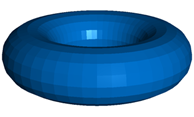
\includegraphics[height=0.35\textheight]{img/simple.png}
	\caption{Результат работы алгоритма простой закраски}
	\label{img:simple-draw}
\end{figure}

Данный метод закраски обладает большим быстродействием, однако все пиксели грани имеют одинаковую интенсивность, и сцена выглядит нереалистично. 
Тем не менее, этот метод крайне прост в реализации и совершенно не требователен к ресурсам.

\subsubsection{Закраска по Гуро}

Метод Гуро устранить дискретность изменения интенсивности и создать иллюзию гладкой криволинейной поверхности.
Он основан на интерполяции интенсивности.

Данный метод отличается от простой закраски тем, что разные точки грани закрашиваются с разными значениями интенсивности.
Для это в каждой вершине грани находится вектор нормали и вычисляется значение интенсивности.
Затем найденные значения интенсивности интерполируются по всем точкам примыкающих граней.
На рисунке~\ref{img:guro} представлен пример работы алгоритма закраски по Гуро.

Закрашивание граней по методу Гуро осуществляется в четыре этапа.
\begin{enumerate}
	\item Вычисляются нормали к каждой грани.
	\item Определяются нормали в вершинах. Нормаль в вершине определяется усреднением нормалей примыкающих граней.
	\item На основе нормалей в вершинах вычисляются значения интенсивностей в вершинах согласно выбранной модели отражения света.
	\item Закрашиваются полигоны граней цветом, соответствующим линейной интерполяции значений интенсивности в вершинах.
\end{enumerate}

\begin{figure}[h]
	\centering
	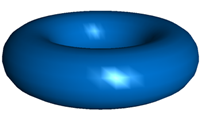
\includegraphics[height=0.35\textheight]{img/guro.png}
	\caption{Результат работы алгоритма закраски по Гуро}
	\label{img:guro}
\end{figure}

Метод Гуро применим для небольших граней, расположенных на значительном расстоянии от источника света. Если же размер грани большой, то расстояние от источника света до центра будет меньше, чем до вершин, и центр грани должен выглядеть ярче, чем ребра. 
Но из-за линейного закона, используемого в интерполяции, метод не позволяет это сделать, поэтому появляются участки с неестественной освещенностью

\subsubsection{Закраска по Фонгу}

Закраска Фонга по своей идее похожа на закраску Гуро, но ее отличие состоит в том, что в методе Гуро по всем точкам полигона интерполируется значения интенсивностей, а в методе Фонга – вектора нормалей, и с их помощью для каждой точки находится значение интенсивности~\cite{roders}.
На рисунке~\ref{img:fong} представлен пример работы алгоритма закраски по Фонгу.

Этапы следующие.
\begin{enumerate}
	\item Определяются нормали к граням.
	\item По нормалям к граням определяются нормали в вершинах. В каждой точке закрашиваемой грани определяется интерполированный вектор нормали.
	\item По направлению векторов нормали определяется цвет точек грани в соответствии с выбранной моделью отражения света.
\end{enumerate}

\begin{figure}[h]
	\centering
	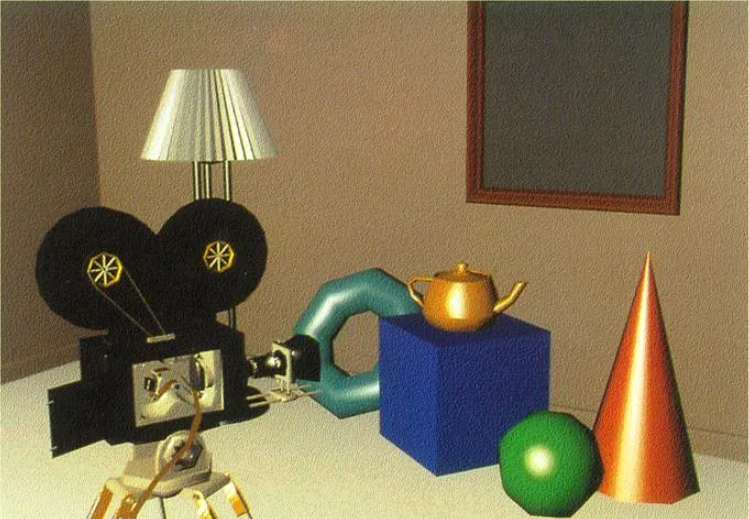
\includegraphics[height=0.35\textheight]{img/fong.png}
	\caption{Результат работы алгоритма закраски по Фонгу}
	\label{img:fong}
\end{figure}

Эта закраска требует больших вычислительных затрат, чем предыдущие, однако она позволяет достигнуть лучшей локальной аппроксимации кривизны поверхности и, следовательно, с ее помощью получается более реалистичное изображение. 

\subsubsection {Выбор алгоритма закраски}

Алгоритм закраски Фонга требует большего числа вычислений по сравнению с другими, однако он дает наиболее реалистичное изображение, в частности зеркальных бликов. В данном курсовом проекте пользователь должен иметь возможность задавать спектральные характеристики объектов, в том числе коэффициенты зеркального отражения и блеска поверхности, поэтому для получения более реалистичной сцены используется метод закраски Фонга.

\subsection{Анализ алгоритма построения теней}

Для генерации теней в данном курсовом проекте используется метод теневых карт. 
Он основан на алгоритме Z-буфера: сначала камера устанавливается на позицию источника освещения и происходит построение сцены с занесением глубин в теневой буфер (карту теней). 
Все точки в этом буфере видимы с точки зрения источника, соответственно они освещены. 
После этого изображение строится уже с позиции наблюдателя, при этом для каждой точки буфера кадра расстояние до источника освещения сравнивается со значением из теневой карты: если это расстояние больше полученного значения из карты, то точка лежит в тени и отображается только с учетом рассеянного света. Иначе точка освещена и происходит расчет ее интенсивности со всеми составляющими освещения. 

Так как используемый источник освещения является точечным, то есть излучающим свет во всех направлениях, то для генерации теней необходимо произвести построение сцены 6 раз для разных направлений камеры: вдоль и против осей OX, OY и OZ. В результате образуется так называемая кубическая карта теней, в которой содержатся значения глубин всех освещенных участков сцены. 

Этот способ генерации теней требует значительного числа вычислений, однако они выполняются только при перестроении сцены, то есть при изменении положения камеры заново вычислять значения в карте теней не нужно. Таким образом метод кубической карты теней позволяет сохранить плавность подачи картинки при перемещении по сцене, поэтому используется в данном курсовом проекте.

\subsection{Анализ моделей освещения}

Все модели освещения делятся на два вида: глобальные и локальные. 
Глобальные модели учитывают возможности отражения и преломления света от объектов, не являющихся прямыми источниками освещения, поэтому они требуют значительных затрат.
Например, прозрачные поверхности должны позволять видеть объекты за ними, на поверхностях возможно появление таких явлений, как
рефлексы.
Глобальные модели освещения основываются на том, что видимость и затенения связаны между собой: яркость точки поверхности определяется распределением яркости по всем остальным поверхностям, видимым из этой точки. 
Так можно моделировать шероховатость и свойства отражения реальных материалов, освещение многократно отраженным светом и связанные с ним цветовые эффекты~\cite{light-model}.

Существуют более простые, локальные модели освещения, которые учитывают только свет от источника. 
Они вычисляют интенсивность, цвет и дальнейшее распределение света на поверхности, но не учитывают перенос света между объектами. 
Изображение формируется в результате отражения, падающего на поверхность объектов света, интенсивность и цвет которого необходимо рассчитать.
Фоновое освещение определяет цвет объекта в тени или при отсутствии явных источников освещения. Его интенсивность постоянна, а также равномерно распределена по всему пространству. 

Выделяют две основные модели локального освещения: модель Ламберта и модель Фонга.

\subsubsection{Модель Ламберта}
Модель Ламберта моделирует идеальное диффузное освещение. Считается, что свет при попадании на поверхность рассеивается равномерно во все стороны.
На рисунке~\ref{img:lambert} показано, что согласно этой модели, освещенность в точке определяется только плотностью света в точке поверхности, а она линейно зависит от косинуса угла падения. 
При этом положение наблюдателя не имеет значения, т.к. диффузно отраженный свет рассеивается равномерно по всем направлениям~\cite{light-model}.

\begin{figure}[h]
	\centering
	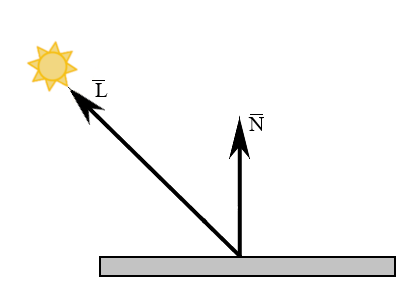
\includegraphics[height=0.3\textheight]{img/lambert.png}
	\caption{Модель освещения Ламберта}
	\label{img:lambert}
\end{figure}

Пусть:
\begin{itemize}
	\item $\overrightarrow L$ --- вектор от точки до источника;
	\item $\overrightarrow N$ --- вектор нормали;
	\item $I$ --- результирующая интенсивность света в точке;
	\item $I_0$ --- интенсивность источника;
	\item $K_d$ --- коэффициент диффузного освещения.
\end{itemize}

Формула расчета интенсивности имеет следующий вид:
\begin{equation}
	\label{eq:lambert}
	I = I_0 \cdot K_d \cdot cos(\overrightarrow L, \overrightarrow N) = I_0 \cdot K_d \cdot (\overrightarrow L, \overrightarrow N) 
\end{equation}
Из формулы (\ref{eq:lambert}) следует главный недостаток модели Ламберта – одинаковая интенсивность во всех точках, принадлежащих одной грани.

Модель Ламберта является одной из самых простых моделей освещения. Данная модель очень часто используется в комбинации других моделей, практически в любой другой модели освещения можно выделить диффузную составляющую. Более-менее равномерная часть освещения (без присутствия какого-либо всплеска) как правило будет представляться моделью Ламберта с определенными характеристиками.

\subsubsection{Модель Фонга}

Модель Фонга – классическая модель освещения. Модель представляет собой комбинацию диффузной составляющей (модели Ламберта) и зеркальной составляющей и работает таким образом, что кроме равномерного освещения на материале может еще появляться блик.
Падающий и отраженный лучи лежат в одной плоскости с нормалью к отражающей поверхности в точке падения, и эта нормаль делит угол между лучами на две равные части как показано на рисунке~\ref{img:fong-light}.

\begin{figure}[h]
	\centering
	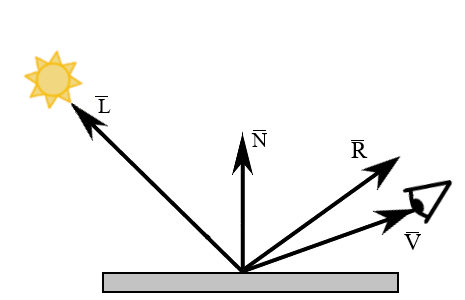
\includegraphics[height=0.3\textheight]{img/phong.png}
	\caption{Модель освещения Фонга}
	\label{img:fong-light}
\end{figure}

Отраженная составляющая освещенности в точке зависит от того, насколько близки направления на наблюдателя и отраженного луча.
Также в модели освещения Фонга используется понятие рассеянного освещения – это константа, которая прибавляется к интенсивности в точке для придания сцене большей реалистичности. 
 
Таким образом, согласно модели Фонга интенсивность к точке складывается будет рассчитываться по формуле: 
\begin{equation}
	\label{eq:simple-model}
	I = I_a + I_d + I_s,
\end{equation}
где $I_a$ --- диффузная составляющая, $I_d$ --- рассеянная  составляющая, $I_s$ --- зеркальная составляющая.
 
\begin{figure}[h]
	\centering
	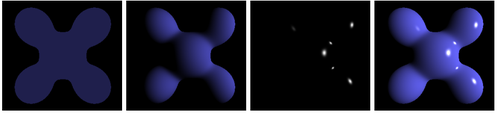
\includegraphics[height=0.15\textheight]{img/phong-model.png}
	\caption{Составляющие модели Фонга (слева направо: рассеянная, диффузная, зеркальная, суммарная)}
	\label{img:fong-model}
\end{figure}

Пусть:
\begin{itemize}
	\item $\overrightarrow R$ --- вектор отраженного луча;
	\item $\overrightarrow V$ --- вектор от точки до наблюдателя;
	\item $I_p$ --- интенсивность рассеянного освещения;
	\item $K_3$ --- коэффициент зеркального освещения;
	\item $K_a$ --- коэффициент рассеянного освещения;
	\item $\alpha$ --- коэффициент блеска.
\end{itemize}
 
Формула для расчета интенсивности для модели Фонга имеет вид:
\begin{equation}
	\label{eq:lambert}
	\begin{aligned}
		I = I_p \cdot K_a  + I_0 \cdot K_d \cdot cos(\overrightarrow L, \overrightarrow N) + I_0 \cdot K_3 \cdot cos^{\alpha}(\overrightarrow R, \overrightarrow V) = \\ = I_p \cdot K_a  + I_0 \cdot K_d \cdot (\overrightarrow L, \overrightarrow N) + I_0 \cdot K_3 \cdot (\overrightarrow R, \overrightarrow V)^{\alpha} 
	\end{aligned}
\end{equation}
 
\subsection*{Вывод}
Подведя итог и проанализировав все вышеописанные алгоритмы методов освещение, можно сделать вывод, что наилучшим алгоритмом для решения задачи будет метод Фонга в сочетании с закраской Фонга, так как он позволяет получить реалистичную картинку с эффектами отражения и преломления лучей. 